% Created by tikzDevice version 0.5.2 on 2011-03-14 15:14:42
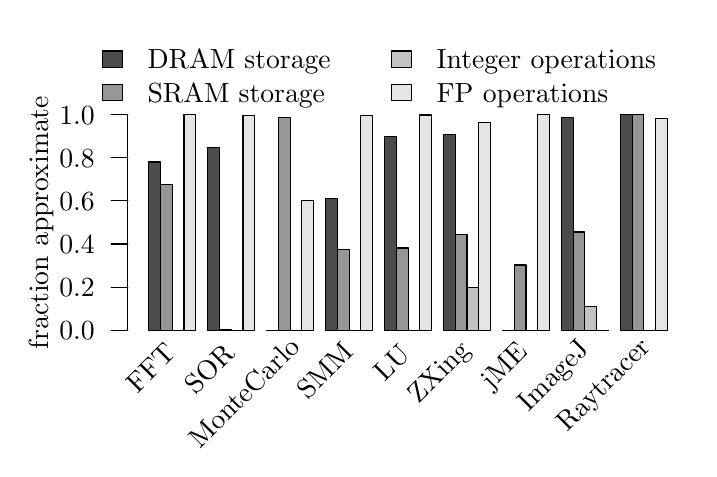
\begin{tikzpicture}[x=1pt,y=1pt]
\draw[color=white,opacity=0] (0,0) rectangle (238.49,151.77);
\begin{scope}
\path[clip] (  0.00,  0.00) rectangle (238.49,151.77);
\definecolor[named]{drawColor}{rgb}{0.18,0.00,0.42}
\definecolor[named]{fillColor}{rgb}{0.45,0.45,0.18}
\definecolor[named]{drawColor}{rgb}{0.00,0.00,0.00}
\definecolor[named]{fillColor}{rgb}{0.30,0.30,0.30}

\draw[color=drawColor,line cap=round,line join=round,fill=fillColor,] ( 43.50, 42.60) rectangle ( 47.76,103.42);
\definecolor[named]{fillColor}{rgb}{0.59,0.59,0.59}

\draw[color=drawColor,line cap=round,line join=round,fill=fillColor,] ( 47.76, 42.60) rectangle ( 52.02, 95.34);
\definecolor[named]{fillColor}{rgb}{0.76,0.76,0.76}

\draw[color=drawColor,line cap=round,line join=round,fill=fillColor,] ( 52.02, 42.60) rectangle ( 56.28, 42.60);
\definecolor[named]{fillColor}{rgb}{0.90,0.90,0.90}

\draw[color=drawColor,line cap=round,line join=round,fill=fillColor,] ( 56.28, 42.60) rectangle ( 60.54,120.53);
\definecolor[named]{fillColor}{rgb}{0.30,0.30,0.30}

\draw[color=drawColor,line cap=round,line join=round,fill=fillColor,] ( 64.81, 42.60) rectangle ( 69.07,108.72);
\definecolor[named]{fillColor}{rgb}{0.59,0.59,0.59}

\draw[color=drawColor,line cap=round,line join=round,fill=fillColor,] ( 69.07, 42.60) rectangle ( 73.33, 42.71);
\definecolor[named]{fillColor}{rgb}{0.76,0.76,0.76}

\draw[color=drawColor,line cap=round,line join=round,fill=fillColor,] ( 73.33, 42.60) rectangle ( 77.59, 42.60);
\definecolor[named]{fillColor}{rgb}{0.90,0.90,0.90}

\draw[color=drawColor,line cap=round,line join=round,fill=fillColor,] ( 77.59, 42.60) rectangle ( 81.85,120.36);
\definecolor[named]{fillColor}{rgb}{0.30,0.30,0.30}

\draw[color=drawColor,line cap=round,line join=round,fill=fillColor,] ( 86.11, 42.60) rectangle ( 90.37, 42.60);
\definecolor[named]{fillColor}{rgb}{0.59,0.59,0.59}

\draw[color=drawColor,line cap=round,line join=round,fill=fillColor,] ( 90.37, 42.60) rectangle ( 94.63,119.67);
\definecolor[named]{fillColor}{rgb}{0.76,0.76,0.76}

\draw[color=drawColor,line cap=round,line join=round,fill=fillColor,] ( 94.63, 42.60) rectangle ( 98.89, 42.60);
\definecolor[named]{fillColor}{rgb}{0.90,0.90,0.90}

\draw[color=drawColor,line cap=round,line join=round,fill=fillColor,] ( 98.89, 42.60) rectangle (103.16, 89.36);
\definecolor[named]{fillColor}{rgb}{0.30,0.30,0.30}

\draw[color=drawColor,line cap=round,line join=round,fill=fillColor,] (107.42, 42.60) rectangle (111.68, 90.22);
\definecolor[named]{fillColor}{rgb}{0.59,0.59,0.59}

\draw[color=drawColor,line cap=round,line join=round,fill=fillColor,] (111.68, 42.60) rectangle (115.94, 71.94);
\definecolor[named]{fillColor}{rgb}{0.76,0.76,0.76}

\draw[color=drawColor,line cap=round,line join=round,fill=fillColor,] (115.94, 42.60) rectangle (120.20, 42.60);
\definecolor[named]{fillColor}{rgb}{0.90,0.90,0.90}

\draw[color=drawColor,line cap=round,line join=round,fill=fillColor,] (120.20, 42.60) rectangle (124.46,120.09);
\definecolor[named]{fillColor}{rgb}{0.30,0.30,0.30}

\draw[color=drawColor,line cap=round,line join=round,fill=fillColor,] (128.72, 42.60) rectangle (132.98,112.64);
\definecolor[named]{fillColor}{rgb}{0.59,0.59,0.59}

\draw[color=drawColor,line cap=round,line join=round,fill=fillColor,] (132.98, 42.60) rectangle (137.25, 72.35);
\definecolor[named]{fillColor}{rgb}{0.76,0.76,0.76}

\draw[color=drawColor,line cap=round,line join=round,fill=fillColor,] (137.25, 42.60) rectangle (141.51, 42.60);
\definecolor[named]{fillColor}{rgb}{0.90,0.90,0.90}

\draw[color=drawColor,line cap=round,line join=round,fill=fillColor,] (141.51, 42.60) rectangle (145.77,120.43);
\definecolor[named]{fillColor}{rgb}{0.30,0.30,0.30}

\draw[color=drawColor,line cap=round,line join=round,fill=fillColor,] (150.03, 42.60) rectangle (154.29,113.43);
\definecolor[named]{fillColor}{rgb}{0.59,0.59,0.59}

\draw[color=drawColor,line cap=round,line join=round,fill=fillColor,] (154.29, 42.60) rectangle (158.55, 77.24);
\definecolor[named]{fillColor}{rgb}{0.76,0.76,0.76}

\draw[color=drawColor,line cap=round,line join=round,fill=fillColor,] (158.55, 42.60) rectangle (162.81, 57.99);
\definecolor[named]{fillColor}{rgb}{0.90,0.90,0.90}

\draw[color=drawColor,line cap=round,line join=round,fill=fillColor,] (162.81, 42.60) rectangle (167.07,117.78);
\definecolor[named]{fillColor}{rgb}{0.30,0.30,0.30}

\draw[color=drawColor,line cap=round,line join=round,fill=fillColor,] (171.33, 42.60) rectangle (175.60, 42.66);
\definecolor[named]{fillColor}{rgb}{0.59,0.59,0.59}

\draw[color=drawColor,line cap=round,line join=round,fill=fillColor,] (175.60, 42.60) rectangle (179.86, 66.20);
\definecolor[named]{fillColor}{rgb}{0.76,0.76,0.76}

\draw[color=drawColor,line cap=round,line join=round,fill=fillColor,] (179.86, 42.60) rectangle (184.12, 42.60);
\definecolor[named]{fillColor}{rgb}{0.90,0.90,0.90}

\draw[color=drawColor,line cap=round,line join=round,fill=fillColor,] (184.12, 42.60) rectangle (188.38,120.57);
\definecolor[named]{fillColor}{rgb}{0.30,0.30,0.30}

\draw[color=drawColor,line cap=round,line join=round,fill=fillColor,] (192.64, 42.60) rectangle (196.90,119.37);
\definecolor[named]{fillColor}{rgb}{0.59,0.59,0.59}

\draw[color=drawColor,line cap=round,line join=round,fill=fillColor,] (196.90, 42.60) rectangle (201.16, 78.13);
\definecolor[named]{fillColor}{rgb}{0.76,0.76,0.76}

\draw[color=drawColor,line cap=round,line join=round,fill=fillColor,] (201.16, 42.60) rectangle (205.42, 51.17);
\definecolor[named]{fillColor}{rgb}{0.90,0.90,0.90}

\draw[color=drawColor,line cap=round,line join=round,fill=fillColor,] (205.42, 42.60) rectangle (209.69, 42.60);
\definecolor[named]{fillColor}{rgb}{0.30,0.30,0.30}

\draw[color=drawColor,line cap=round,line join=round,fill=fillColor,] (213.95, 42.60) rectangle (218.21,120.55);
\definecolor[named]{fillColor}{rgb}{0.59,0.59,0.59}

\draw[color=drawColor,line cap=round,line join=round,fill=fillColor,] (218.21, 42.60) rectangle (222.47,120.56);
\definecolor[named]{fillColor}{rgb}{0.76,0.76,0.76}

\draw[color=drawColor,line cap=round,line join=round,fill=fillColor,] (222.47, 42.60) rectangle (226.73, 42.60);
\definecolor[named]{fillColor}{rgb}{0.90,0.90,0.90}

\draw[color=drawColor,line cap=round,line join=round,fill=fillColor,] (226.73, 42.60) rectangle (230.99,119.07);
\end{scope}
\begin{scope}
\path[clip] (  0.00,  0.00) rectangle (238.49,151.77);
\definecolor[named]{drawColor}{rgb}{0.18,0.00,0.42}
\definecolor[named]{fillColor}{rgb}{0.45,0.45,0.18}
\definecolor[named]{drawColor}{rgb}{0.00,0.00,0.00}

\draw[color=drawColor,line cap=round,line join=round,fill opacity=0.00,] ( 36.00, 42.60) -- ( 36.00,120.57);

\draw[color=drawColor,line cap=round,line join=round,fill opacity=0.00,] ( 36.00, 42.60) -- ( 30.00, 42.60);

\draw[color=drawColor,line cap=round,line join=round,fill opacity=0.00,] ( 36.00, 58.19) -- ( 30.00, 58.19);

\draw[color=drawColor,line cap=round,line join=round,fill opacity=0.00,] ( 36.00, 73.79) -- ( 30.00, 73.79);

\draw[color=drawColor,line cap=round,line join=round,fill opacity=0.00,] ( 36.00, 89.38) -- ( 30.00, 89.38);

\draw[color=drawColor,line cap=round,line join=round,fill opacity=0.00,] ( 36.00,104.97) -- ( 30.00,104.97);

\draw[color=drawColor,line cap=round,line join=round,fill opacity=0.00,] ( 36.00,120.57) -- ( 30.00,120.57);

\node[color=drawColor,anchor=base east,inner sep=0pt, outer sep=0pt, scale=  1.00] at ( 24.00, 39.16) {0.0%
};

\node[color=drawColor,anchor=base east,inner sep=0pt, outer sep=0pt, scale=  1.00] at ( 24.00, 54.75) {0.2%
};

\node[color=drawColor,anchor=base east,inner sep=0pt, outer sep=0pt, scale=  1.00] at ( 24.00, 70.34) {0.4%
};

\node[color=drawColor,anchor=base east,inner sep=0pt, outer sep=0pt, scale=  1.00] at ( 24.00, 85.94) {0.6%
};

\node[color=drawColor,anchor=base east,inner sep=0pt, outer sep=0pt, scale=  1.00] at ( 24.00,101.53) {0.8%
};

\node[color=drawColor,anchor=base east,inner sep=0pt, outer sep=0pt, scale=  1.00] at ( 24.00,117.12) {1.0%
};

\node[rotate= 90.00,color=drawColor,anchor=base,inner sep=0pt, outer sep=0pt, scale=  1.00] at (  7.20, 81.58) {fraction approximate%
};
\end{scope}
\begin{scope}
\path[clip] (  0.00,  0.00) rectangle (238.49,151.77);
\definecolor[named]{drawColor}{rgb}{0.18,0.00,0.42}
\definecolor[named]{fillColor}{rgb}{0.45,0.45,0.18}
\definecolor[named]{drawColor}{rgb}{0.00,0.00,0.00}
\definecolor[named]{fillColor}{rgb}{0.30,0.30,0.30}

\draw[color=drawColor,line cap=round,line join=round,fill=fillColor,] ( 26.93,143.53) rectangle ( 34.13,137.53);
\definecolor[named]{fillColor}{rgb}{0.59,0.59,0.59}

\draw[color=drawColor,line cap=round,line join=round,fill=fillColor,] ( 26.93,131.53) rectangle ( 34.13,125.53);
\definecolor[named]{fillColor}{rgb}{0.76,0.76,0.76}

\draw[color=drawColor,line cap=round,line join=round,fill=fillColor,] (131.39,143.53) rectangle (138.59,137.53);
\definecolor[named]{fillColor}{rgb}{0.90,0.90,0.90}

\draw[color=drawColor,line cap=round,line join=round,fill=fillColor,] (131.39,131.53) rectangle (138.59,125.53);

\node[color=drawColor,anchor=base west,inner sep=0pt, outer sep=0pt, scale=  1.00] at ( 43.13,137.09) {DRAM storage%
};

\node[color=drawColor,anchor=base west,inner sep=0pt, outer sep=0pt, scale=  1.00] at ( 43.13,125.09) {SRAM storage%
};

\node[color=drawColor,anchor=base west,inner sep=0pt, outer sep=0pt, scale=  1.00] at (147.59,137.09) {Integer operations%
};

\node[color=drawColor,anchor=base west,inner sep=0pt, outer sep=0pt, scale=  1.00] at (147.59,125.09) {FP operations%
};

\node[rotate= 45.00,color=drawColor,anchor=base east,inner sep=0pt, outer sep=0pt, scale=  1.00] at ( 53.76, 33.80) {FFT%
};

\node[rotate= 45.00,color=drawColor,anchor=base east,inner sep=0pt, outer sep=0pt, scale=  1.00] at ( 75.10, 33.83) {SOR%
};

\node[rotate= 45.00,color=drawColor,anchor=base east,inner sep=0pt, outer sep=0pt, scale=  1.00] at ( 98.59, 36.02) {MonteCarlo%
};

\node[rotate= 45.00,color=drawColor,anchor=base east,inner sep=0pt, outer sep=0pt, scale=  1.00] at (117.93, 34.06) {SMM%
};

\node[rotate= 45.00,color=drawColor,anchor=base east,inner sep=0pt, outer sep=0pt, scale=  1.00] at (138.52, 33.34) {LU%
};

\node[rotate= 45.00,color=drawColor,anchor=base east,inner sep=0pt, outer sep=0pt, scale=  1.00] at (160.07, 34.96) {ZXing%
};

\node[rotate= 45.00,color=drawColor,anchor=base east,inner sep=0pt, outer sep=0pt, scale=  1.00] at (180.82, 34.40) {jME%
};

\node[rotate= 45.00,color=drawColor,anchor=base east,inner sep=0pt, outer sep=0pt, scale=  1.00] at (203.01, 35.28) {ImageJ%
};

\node[rotate= 45.00,color=drawColor,anchor=base east,inner sep=0pt, outer sep=0pt, scale=  1.00] at (225.12, 36.09) {Raytracer%
};
\end{scope}
\end{tikzpicture}
